\chapter{Evaluation of New Sensor
\label{chap:8}}

Over the course of this program, two primary load cell designs were tested.
The first design had two electrodes separated by a thin, 25 $\mu$m, layer of polyimide.
The second design had a single electrode coated in soldermask 
and attached to a thicker, 100 $\mu$m, layer of polyimide.
Both designs were tested in a load frame and in full scale rock cutting tests.
The results from both kinds of tests for both sensors are shown below.

\subsection{Load Frame Testing
\label{compare1}}

Comparable XY plots are shown for both the first and second design
in \ref{fig:xycompare}. The first design is the ``Dynamic Flex Configuration'' 
and the second is the ``Air Gap Configuration''.
One thing that was the same for both sensor designs was the steel case. This case
is made of stainless steel, and has a measured stiffness of around 780 MN/m. 
The walls of this case provide the stiffness and repeatable deformation characteristics
needed for a robust sensor. This case also provides protection to the sensing element by
shielding it from debris and electromagnetic interference.

In can be seen in the load frame testing graphs that the air gap design
gives a much cleaner measurement, in that it has much less noise and reduced hysteresis.
The plastic deformation of the sensor case is about the same magnitude for both designs.
The air gap design is also more sensitive in the load frame test than the dynamic flex cell configuration.
Both sensors saw their sensitivity increase when used in the rock cutting tests.

\subsection{Rock Cut Testing
\label{compare2}}

The first design was already very thin when it went into the rock cutting test.
The nonlinear deformation characteristics of the thin film made it difficult to determine
cutting forces, but still allowed frequency analysis for determining material type and tool wear.
The second design ultimately altered to the ``Crushed Gap Configuration'' when used for rock cutting.
This final form had even greater sensitivity and linearity, which allowed estimation of cutting forces.

Measurements for individual sensor channels and the measured 
and estimated forces are shown in \ref{fig:sense_chans}.
When attempting to estimate the rock cutting forces to determine material type and tool wear, 
the problem can be relaxed to estimating average cutting force, as the differences in 
cutting force between the conditions are great.
The cutting force bandwidth was limited to 10 Hz for the study, as this is believed to still
provide an adequate response time while providing good averaging.

\begin{figure}[ht]
\centering
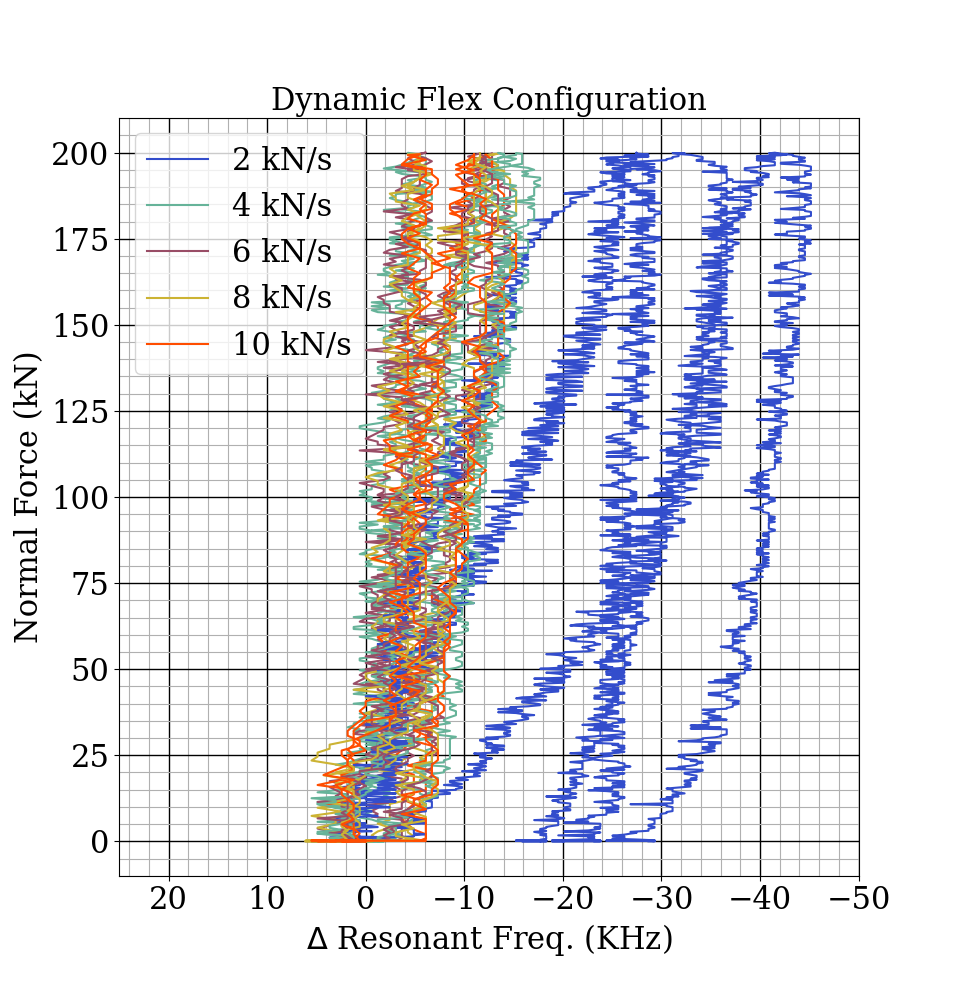
\includegraphics[width=3.0in]{ch8_flexcell.png}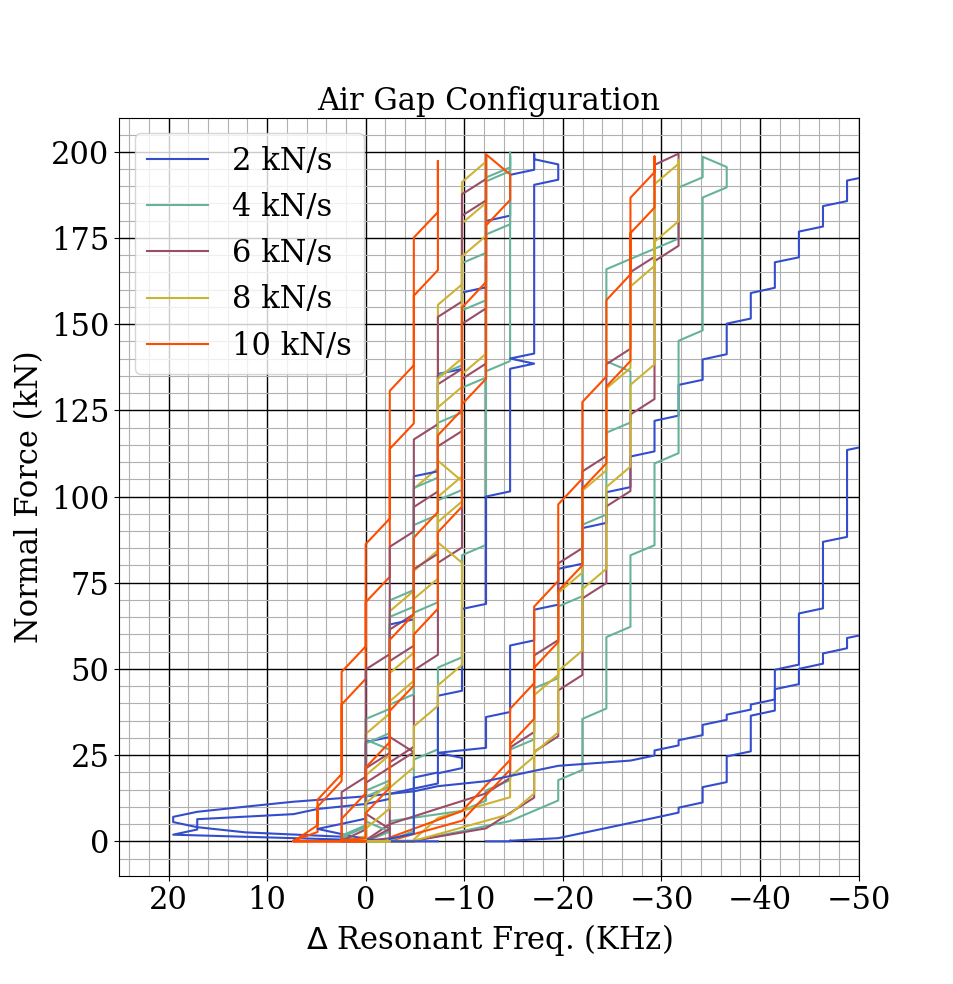
\includegraphics[width=3.0in]{ch8_airgap.png}
\caption{
Comparison of original design, left, and improved design, right.
The original design was noisy, had slightly less initial plastic deformation,
and similar sensitivity when compared to the improved ``Air Gap Configuration''.
The air gap design had much better repeatability and less hysteresis in comparison 
to the original.
The air gap design ultimately became more sensitive when used in the rock cutting tests.
}
\label{fig:xycompare}
\end{figure}

\begin{figure}[h]
\centering
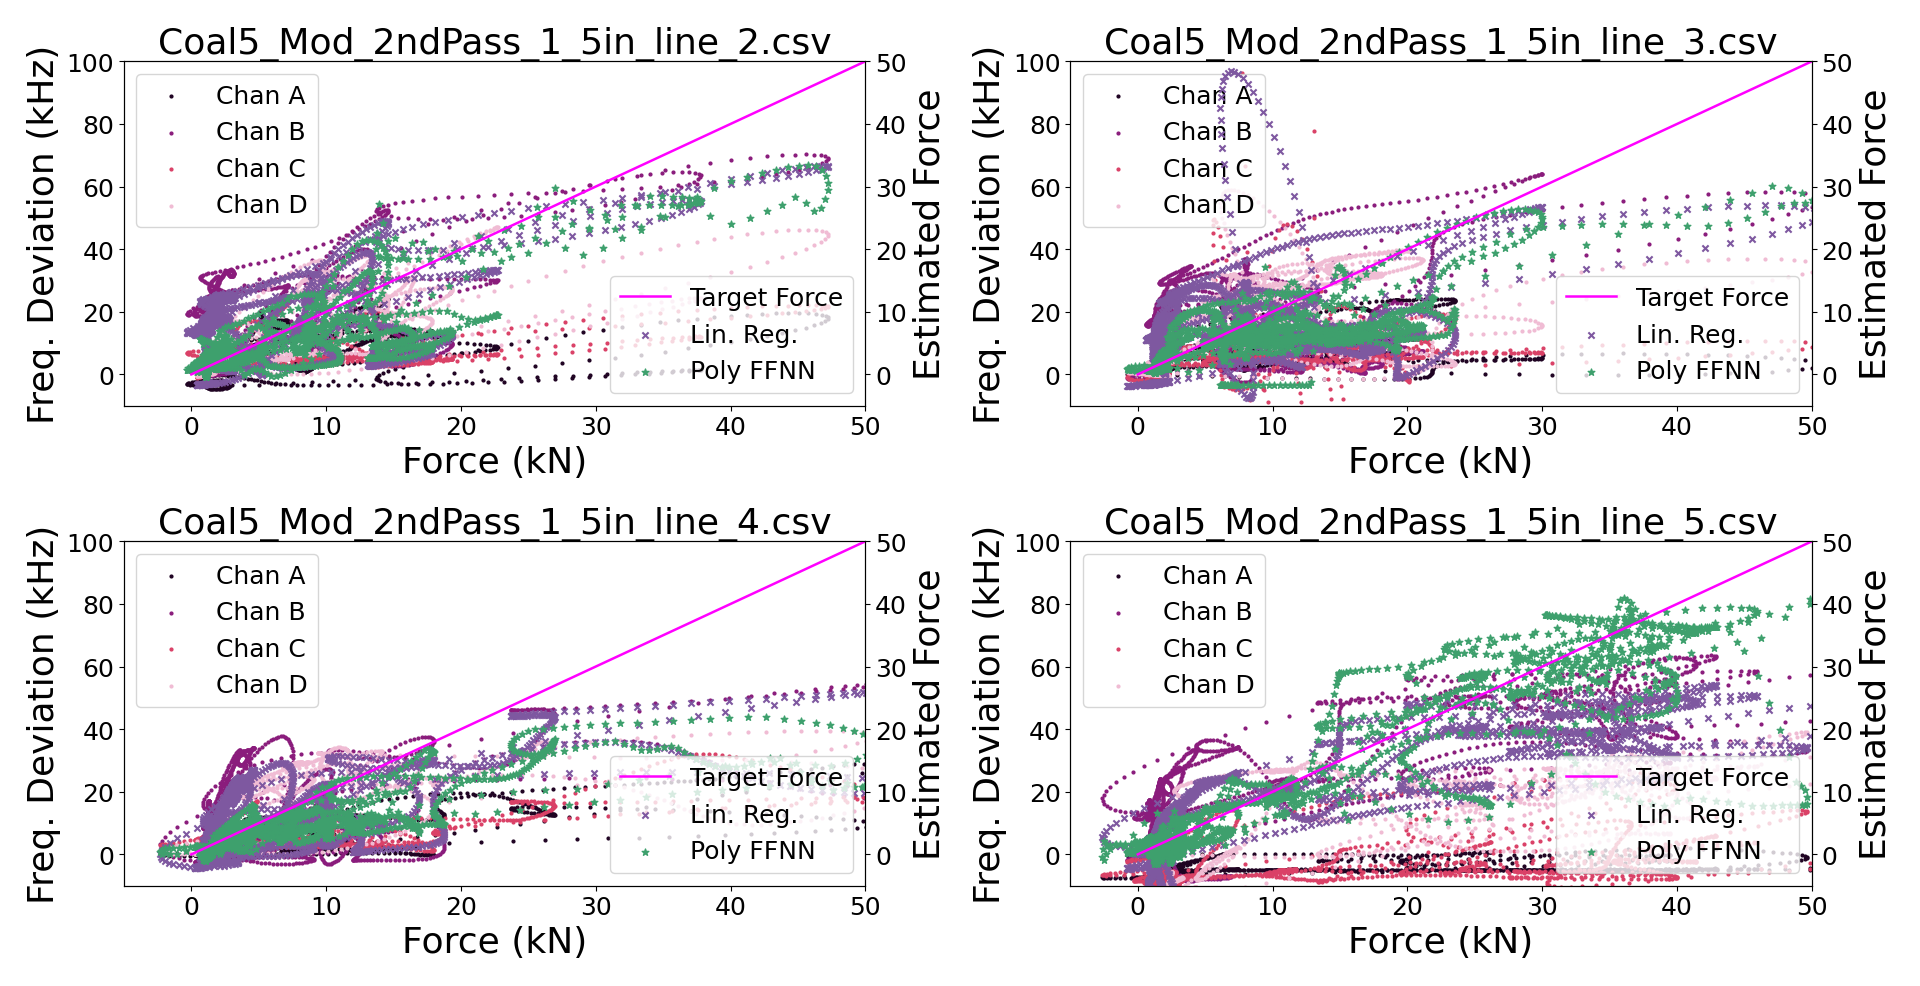
\includegraphics[width=5.5in]{ch8_sense_vals.png}
\caption{
The individual channel measurements and the resulting force predictions for a few choice cuts,
using the ``Crushed Gap Configuration'' of the second sensor design.
The change in resonant frequency from the initial value is plotted versus the target force
for each sensing channel in the sensor. The resulting force estimate provided by both the 
linear regression and the neural network using the 2nd order polynomial expansion are shown.
Ideal performance is shown along the magenta line. 
The neural network method is able to untangle some of the non-linearity in the response.
The performance of the neural network is comparable to the strictly linear model.
The sensor is not completely linear, but can still provide useful measurements using a linear model.
}
\label{fig:sense_chans}
\end{figure}

By averaging the cutting force, the individual rock chipping forces are lost.
These forces are averaged together to form a measurement which varies less with time.
The high frequency rock chipping forces are correlated to rock material type and tool wear 
by their frequency. The average magnitude of these forces is of interest when attempting 
to determine specific energy of a particular tool wear and rock material type setup.

Force on the cutting tool is determined by the tool geometry and the material.
The force is also influenced by the dynamics of the machine.
The physical sensor system also has dynamics, and depending on the model, 
these dynamics can be non-stationary.
The first design that was tested had non-linear, non-stationary dynamics.
The second design was more linear and the bias could be tracked and compensated.

The nonlinear dynamics of the first design caused the vibrational modes to shift
in ways that could not be captured completely with linear models.
The sensor response was not chaotic, and it could still be predicted.
In general, the thin film allows low frequencies and also very high frequencies to pass.
It is possible that energy from some frequencies is moved into others, and there
are other frequencies which are clearly blocked by the membrane.

The follow up air gap design could work for applications with more gentle load profiles,
but considering that the gap will be closed when exposed to rock cutting forces 
means that this aspect of the design is unnecessary. The first sensor design
has a high bandwidth due to its thin film. 
High bandwidth sensing is good for frequency analysis methods.
More linear and robust sensors are generally bulkier, but at the cost of sensitivity.
By starting with a thick polyimide film and allowing it to be compressed during the application,
 a robust sensor that is stiffer and more sensitive than the original design is achieved.

The first design used in this research was very nonlinear, so determining forces with the measurements
did not give useful results. The second design was much more linear in comparison, and was
able to be used to give force measurements.
The seconds design was still nonlinear, but the non-linearities were able to be either ignored in the linear
model case or measured and compensated in the neural network case.
Both capacitive load cell designs were suitable for material and wear classification, although the latter design
was only used to show force measurements. Use of these measurements for rock type and tool wear classification
would be trivial using the classification methods shown in this work.

